\documentclass[a4paper, 12pt]{article}
% packages
\usepackage{amssymb}
\usepackage[fleqn]{mathtools}
\usepackage{tikz}
\usepackage{enumerate}
\usepackage{bussproofs}
\usepackage{xcolor}
\usepackage[margin=1.3cm]{geometry}
\usepackage{logicproof}
\usepackage{diagbox}
\usepackage{listings}
\usepackage{lstautogobble}
\usepackage{hyperref}

% code listing
\lstdefinestyle{main}{
    numberstyle=\tiny,
    breaklines=true,
    showspaces=false,
    showstringspaces=false,
    tabsize=2,
    numbers=left,
    basicstyle=\ttfamily,
    columns=fixed,
    fontadjust=true,
    basewidth=0.5em,
    autogobble,
    xleftmargin=3.0ex,
    mathescape=true
}
\newcommand{\dollar}{\mbox{\textdollar}} %
\lstset{style=main}

% augmented matrix
\makeatletter
\renewcommand*\env@matrix[1][*\c@MaxMatrixCols c]{%
\hskip -\arraycolsep
\let\@ifnextchar\new@ifnextchar
\array{#1}}
\makeatother

% ceiling / floor
\DeclarePairedDelimiter{\ceil}{\lceil}{\rceil}
\DeclarePairedDelimiter{\floor}{\lfloor}{\rfloor}

% custom commands
\newcommand{\indefint}[2]{\int #1 \, \mathrm{d}#2}
\newcommand{\defint}[4]{\int_{#1}^{#2} #3 \, \mathrm{d}#4}
\newcommand{\dif}[2]{\frac{\mathrm{d}#1}{\mathrm{d}#2}}
\newcommand{\limit}[2]{\displaystyle{\lim_{#1 \to #2}}}
\newcommand{\summation}[3]{\sum\limits_{#1}^{#2} #3}
\newcommand{\intbracket}[3]{\left[#3\right]_{#1}^{#2}}

\newcommand{\powerset}[0]{\wp}
\renewcommand{\emptyset}[0]{\varnothing}

\newcommand{\unaryproof}[2]{\AxiomC{#1} \UnaryInfC{#2} \DisplayProof}
\newcommand{\binaryproof}[3]{\AxiomC{#1} \AxiomC{#2} \BinaryInfC{#3} \DisplayProof}
\newcommand{\trinaryproof}[4]{\AxiomC{#1} \AxiomC{#2} \AxiomC{#3} \TrinaryInfC{#4} \DisplayProof}

% no indent
\setlength\parindent{0pt}

% reasoning proofs
\usepackage{ltablex}
\usepackage{environ}
\keepXColumns
\NewEnviron{reasoning}{
    \begin{tabularx}{\textwidth}{rlX}
        \BODY
    \end{tabularx}
}
\newcommand{\proofline}[3]{$(#1)$ & $#2$ & \hfill #3 \smallskip \\}
\newcommand{\proofarbitrary}[1]{& take arbitrary $#1$ \smallskip \\}
\newcommand{\prooftext}[1]{\multicolumn{3}{l}{#1} \smallskip \\}
\newcommand{\proofmath}[3]{$#1$ & = $#2$ & \hfill #3 \smallskip \\}
\newcommand{\prooftherefore}[1]{& $\therefore #1$ \smallskip \\}
\newcommand{\proofbc}[0]{\prooftext{\textbf{Base Case}}}
\newcommand{\proofis}[0]{\prooftext{\textbf{Inductive Step}}}

% actual document
\begin{document}
    \section*{CO113 - Architecture}
        \subsection*{Prelude}
            The content discussed here is part of CO113 - Architecture (Computing MEng); taught by Wayne Luk, and Jana Giceva, in Imperial College London during the academic year 2018/19. The notes are written for my personal use, and have no guarantee of being correct (although I hope it is, for my own sake). This should be used in conjunction with the lecture slides, \href{https://www.youtube.com/playlist?list=PL0oekSefhQVJdk0hSRu6sZ2teWM740NtL}{\textit{The Hardware/Software Interface Class by Luis Ceze and Gaetano Borriello}} on YouTube, and \textit{Computer Organization and Design : The Hardware / Software Interface (Fifth Edition)} (chapters 1 to 4, and appendices B, and D), by Patterson, D., and Hennessy, J.
            \medskip

            The second part of the course seems to be covered in sufficient detail by the YouTube playlist, which is where the majority of the information in these notes will come from.
        \subsection*{Lecture 1 \hfill P\&H 62-120}
            Computer architecture is a combination of ISA (instruction set architecture), and machine organisation. We can see the ISA as an interface between the high level software, and the capabilities of the physical hardware components.The benefit of having the ISA is that a piece of software can be compiled into an instruction set, and then be reused on different hardware. For example, near identical versions of the x86 instruction set are used in Intel, and AMD chips despite the two having drastically different internal designs. On the other hand, microarchitecture, or computer organisation, is the the way a given ISA is implemented in a particular processor. This comes with the additional benefit that code doesn't need to be reimplemented even if there is a drastic change in the future for the microarchitecture / machine organisation.
            \medskip

            There are two design approaches, both of which have their benefits, and drawbacks;
            \begin{itemize}
                \itemsep0em
                \item Complex Instruction Set Computers (CISC)
                    \subitem The programs run on this design are closer to the high-level languages that we program in; which means that the compilers used are simpler. This is possible due to the decreasing size of transistors, and thus the increased number of gates on a chip. Programs on this instruction set tend to be smaller, as code can be represented in fewer instructions, thus saving storage.
                \item Reduced Instruction Set Computers (RISC)
                    \subitem On the other hand, the programs running on this instruction set are closer to machine code, due to the smaller range of instructions. A more powerful, better optimised, compiler will be required. Additionally, the programs here are faster, since they have simpler instructions - but they may require more instructions to achieve what a CISC can do in one, thus there may be a trade-off. It's also easier to build a chip with less instructions, which leads to lower development costs. Due to the smaller physical size of the chips, we can not only fit multiple chips together, but also use the space for memory, since accessing memory outside of the chip is very slow (compared to the high-speed registers nearby).
            \end{itemize}
            In this course, we will be working mostly on a MIPS processor. Generally, the instructions consist of an opcode, which is what it does, and an operand (which includes the registers, memory locations, and data). This should be fairly similar to the very end of \textbf{CO112 - Hardware}. The design principle for RISCs is that the processor should have good performance, and be relatively simple to implement. In MIPS, there are 3 main types of instructions; R (register), I (immediate), and J (jump), all of which have a fixed size of 32 bits.
            \medskip

            MIPS is representative of modern RISC architectures, and has 32 registers, each being able to store 32-bit data. The registers are named \$0..\$31, with \$0 being typically wired to ground (logic 0), and the others being used for general-purpose storage. MIPS is known as a register-register, or load-store architecture, which means that there are two different sets of instructions; one that is extremely fast, and works between registers, and another set working with memory access, which tends to be slower. The goal is to minimise memory access, as accessing data from memory tends to be much slower than accessing memory located in the registers on the chip. Here are some examples of these instructions;
            \begin{itemize}
                \itemsep0em
                \item register-register
                    \subitem \texttt{add \$1, \$2, \$3} \hfill reg1 = reg2 + reg3
                \item load-store
                    \subitem \texttt{lw \$8, Astart(\$19)} \hfill reg8 = M[Astart + reg19]
            \end{itemize}
            R-type instructions can be used for arithmetic, comparisons, logical operations, etc. and have a general format as follows (the example describes \texttt{add \$8, \$17, \$18}). It's important to note that we have an additional 6 bits at the end for the function, since having a 6-bit opcode only leaves us 64 ($2^6$) instructions, which is quite limited even for a RISC instruction set. In addition, the shift amount specifies the amount of bits to shift, if it was a shift instruction, however it's redundant in this case;
            \begin{center}
                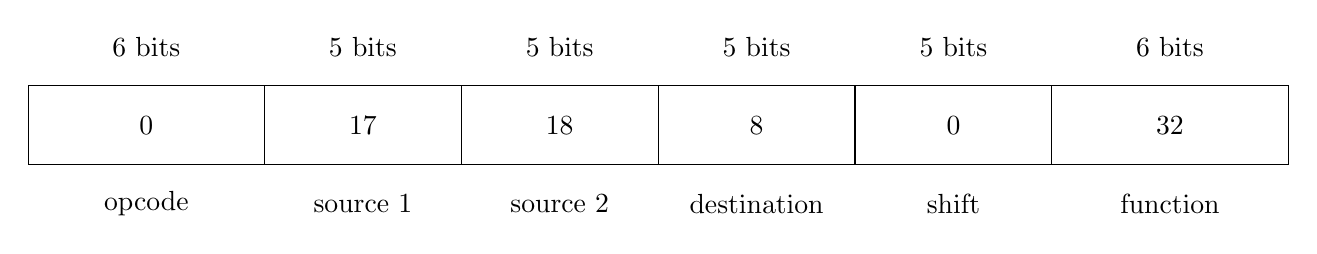
\begin{tikzpicture}
                    \draw
                    (0, 0) -- (16, 0) -- (16, -1) -- (0, -1) -- cycle;

                    \draw
                    (3, 0) -- (3, -1)
                    (5.5, 0) -- (5.5, -1)
                    (8, 0) -- (8, -1)
                    (10.5, 0) -- (10.5, -1)
                    (13, 0) -- (13, -1);

                    \node[] () at (1.5, -0.5) {0};
                    \node[] () at (4.25, -0.5) {17};
                    \node[] () at (6.75, -0.5) {18};
                    \node[] () at (9.25, -0.5) {8};
                    \node[] () at (11.75, -0.5) {0};
                    \node[] () at (14.5, -0.5) {32};

                    \node[] () at (1.5, 0.5) {6 bits};
                    \node[] () at (4.25, 0.5) {5 bits};
                    \node[] () at (6.75, 0.5) {5 bits};
                    \node[] () at (9.25, 0.5) {5 bits};
                    \node[] () at (11.75, 0.5) {5 bits};
                    \node[] () at (14.5, 0.5) {6 bits};

                    \node[] () at (1.5, -1.5) {opcode};
                    \node[] () at (4.25, -1.5) {source 1};
                    \node[] () at (6.75, -1.5) {source 2};
                    \node[] () at (9.25, -1.5) {destination};
                    \node[] () at (11.75, -1.5) {shift};
                    \node[] () at (14.5, -1.5) {function};
                \end{tikzpicture}
            \end{center}
            I-type instructions are used for memory access, conditional branching, or arithmetic with constants. An example of doing addition with constants is \texttt{addi \$1, \$2, 100}, which does reg1 = reg2 + 100. The example displayed below is \texttt{lw \$8, Astart(\$19)}, which does reg8 = M[Astart + reg19].
            \begin{center}
                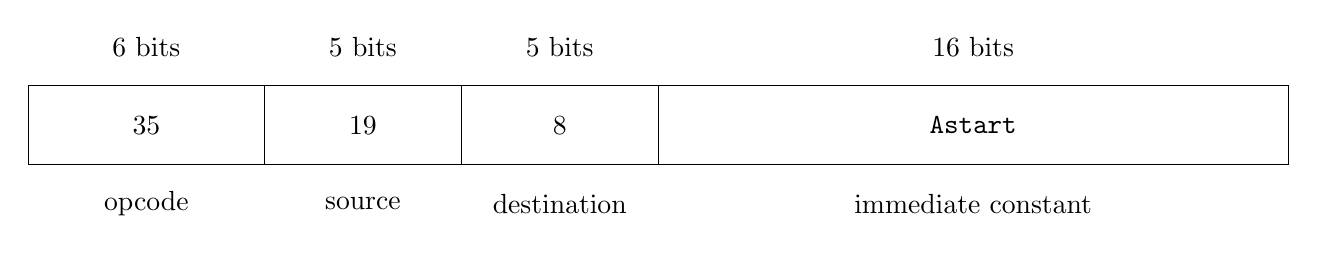
\begin{tikzpicture}
                    \draw
                    (0, 0) -- (16, 0) -- (16, -1) -- (0, -1) -- cycle;

                    \draw
                    (3, 0) -- (3, -1)
                    (5.5, 0) -- (5.5, -1)
                    (8, 0) -- (8, -1);

                    \node[] () at (1.5, -0.5) {35};
                    \node[] () at (4.25, -0.5) {19};
                    \node[] () at (6.75, -0.5) {8};
                    \node[] () at (12, -0.5) {\texttt{Astart}};

                    \node[] () at (1.5, 0.5) {6 bits};
                    \node[] () at (4.25, 0.5) {5 bits};
                    \node[] () at (6.75, 0.5) {5 bits};
                    \node[] () at (12, 0.5) {16 bits};

                    \node[] () at (1.5, -1.5) {opcode};
                    \node[] () at (4.25, -1.5) {source};
                    \node[] () at (6.75, -1.5) {destination};
                    \node[] () at (12, -1.5) {immediate constant};
                \end{tikzpicture}
            \end{center}
            Finally J-type instructions are jump to instructions in memory, for example, \texttt{j 1236} would be an unconditional jump to the instruction at address 1236. An unconditional jump has the following format;
            \begin{center}
                \begin{tikzpicture}
                    \draw
                    (0, 0) -- (16, 0) -- (16, -1) -- (0, -1) -- cycle;

                    \draw
                    (3, 0) -- (3, -1);

                    \node[] () at (1.5, -0.5) {2};
                    \node[] () at (9.5, -0.5) {1236};

                    \node[] () at (1.5, 0.5) {6 bits};
                    \node[] () at (9.5, 0.5) {26 bits};

                    \node[] () at (1.5, -1.5) {opcode};
                    \node[] () at (9.5, -1.5) {memory location};
                \end{tikzpicture}
            \end{center}
            However, we can also have jump instructions, which are I-type, or R-type, for example \texttt{bne \$19, \$20, Label} is an I-type instruction, where the program jumps to \texttt{Label} if registers 19, and 20 aren't equal. An R-type example would be \texttt{jr \$ra}, where it jumps to the address in register ra.

            Consider the following program, and its equivalent in machine code, the registers are labeled in alphabetical order (reg16 = f, reg20 = j, etc);
            \begin{lstlisting}
                if (i == j) {
                  f = g + h;
                } else {
                  f = g - h;
                }

                      bne $\dollar$19, $\dollar$20, Else # if i $\neq$ j goto Else
                      add $\dollar$16, $\dollar$17, $\dollar$18     # f = g + h
                      j   Exit           # goto Exit
                Else: sub $\dollar$16, $\dollar$17, $\dollar$18     # f = g - h
                Exit:
            \end{lstlisting}
            Since we only have two types of conditional branches, \texttt{bne}, and \texttt{beq}, we need \texttt{slt}, which does the following - \texttt{slt \$1, \$16, \$17}, if reg16 $<$ reg17, then it sets reg1 to 1, otherwise it's set to 0. Then, we can use \texttt{bne}, with \texttt{\$0}, since reg0 is always set to logic 0.
        \subsection*{Lecture 2 \hfill P\&H 28-53}
            One of the questions raised in this lecture is the following; "Is a 20\% cheaper processor, with the same performance good enough?". While this may seem straightforward, from a consumer's perspective, it's important to note that a consumer has instant gratification from buying a product, but developing one would take time. In this time, competitors are also trying to improve on their product, and as such you can't just know the price, and performance of a competitor's product \textbf{now}, but you also need to predict the improvement.
            \medskip

            CPI is the \textbf{average} number of clock cycles required per instruction. Note that it's the average, because some instructions may take more cycles to complete. For a given program $P$, we can get the number of cycles required for $P$ by doing the number of instructions in $P$, multiplied by the CPI. The execution time for $P$ is the number of cycles in $P$, multiplied by the clock cycle time (which is $\frac{1}{\text{clock speed}}$). Assuming that for a set of programs $P_1$, ..., $P_n$, the workload is equal, we can calculate the average execution time for the set by taking the mean of the execution times.
            \subsubsection*{Example}
                Consider two machines, $M_1$, and $M_2$, which implement the same instruction set that has 2 classes of instructions; $A$, and $B$. The CPI for $M_1$ on class $A$ is $A_1$, $B$, is $B_1$, and the same for $M_2$. The clock speed of $M_1$ is $C_1$ MHz, and similar for $M_2$. If we were to compare their peak and average performance of $N$ instructions, half of which are of class $A$, and the other half of class $B$, we'd need to find the ratio of execution times.
                \medskip

                In order to find the peak performance of $N$ instructions for $M_1$ (let it be $P_{P1}$), we take the clock cycle time (which is $\frac{1}{C_1}$, multiply it by the number of instructions $N$, miltiply it by the \textbf{minimum} CPI for $M_1$ (which would be min($A_1$, $B_1$)), we'd get $\frac{N(\text{min}(A_1, B_1))}{C_1}$. To compare the two, we take $\frac{P_{P1}}{P_{P2}} = \frac{\text{min}(A_1, B_1) \cdot C_2}{\text{min}(A_2, B_2) \cdot C_1}$.
                \medskip

                We do a similar process for finding the average performance, let it be $P_{A1}$, but instead of multiplying it by the minimum CPI, we take the average, hence we multiply by $\frac{A_1 + B1}{2}$. To compare the two, we take $\frac{P_{A1}}{P_{A2}} = \frac{(A_1 + B_1) \cdot C_2}{(A_2 + B_2) \cdot C_1}$.
                \medskip

                Our goal is to minimize the execution time, which is to minimise $\text{instruction count} \times \text{CPI} \times \text{cycle time}$. Consider this example, comparing SUN 68000, and their newer SUN RISC. In the RISC device, there are 25\% more instructions, and the cycle time is 50\% longer. However, the CPI is much lower, as the instructions are simpler, thus requiring less cycles. The price has increased, but the performance has doubled.
                \begin{center}
                    \begin{tabular}{l|l|l}
                        & SUN 68000 & SUN RISC \\
                        \hline
                        Instruction Count Ratio & 1.0 & 1.25 \\
                        Cycle time & 40ns & 60ns \\
                        CPI & 5.0 - 7.0 & 1.3 - 1.7 \\
                        Execution Time Ratio & 2 & 1 \\
                        Price Ratio & 1 & 1.1 - 1.2
                    \end{tabular}
                \end{center}
                The processor time is measured by the seconds per program, which is calculated as follows; $\frac{\text{time}}{\text{program}} = \frac{\text{instructions}}{\text{program}} \cdot \frac{\text{cycles}}{\text{instruction}} \cdot \frac{\text{time}}{\text{cycle}}$.
            \subsubsection*{RISC}
                Regarding the principles of RISC instruction set design, the common cases should be optimised, thus reducing the CPI. A small number of general purpose registers (32 in MIPS), simplifies things, and allows the design to be more adaptable to new technologies. The smaller chip size allows for a higher yield, thus reducing the cost of production. On the other hand, the lower number of instructions increases the code size, and smarter compilers are needed, since the instructions are further away from the software level than with a CISC instruction set.
            \subsubsection*{Performance Trends}
                In 2004, the trend in power usage hit a peak, due to heat not being able to be removed from the chip at a reasonable rate. The voltage also cannot be reduced further, which is why the trends seemed to have become flat. $P = C \cdot V^2 \cdot F$, where $P$ is power, $C$ is capacitive load, $V$ is voltage, and $F$ is frequency.
                \medskip

                Other than just increasing clock speed, performance can be increased in other ways; including faster local storage, concurrent execution, and newer technologies. Implementning on-chip caches allows for faster execution due to the faster memory closer to the chip, which would be a significant improvement compared to fetching from RAM. Concurrent execution can be achieved by multiple function units (super scalar), a pipeline execution, or multiple instruction streams (multi-threading). Newer technologies, such as GPUs can also be used for specialised loads.
            \subsubsection*{Benchmarking}
                There are a number of ways of benchmarking, each with their benefits, and drawbacks as follows;
                \begin{center}
                    \begin{tabular}{l|l|l}
                        method & pros & cons \\
                        \hline
                        actual target workload & representative & very specific, not portable \\
                        & & difficult to measure \\
                        & & hard to identify problems \\
                        \hline
                        full benchmarks & portable & less representative \\
                        & widespread usage & \\
                        \hline
                        kernel benchmarks & easy to use & peak is not representative \\
                        & used early in design cycle & \\
                        & identify peak performance &
                    \end{tabular}
                \end{center}
        \subsection*{Lecture 3}
            Considering the software side of parallelism; we have parallel requests, parallel threads, parallel instructions, and parallel data. Parallel threads schedule tasks; for example if you have an instruction that takes longer to process since it has to read from main memory, or wait for another resource, another task can be scheduled to run during this time. Since a processor core has multiple functional units, instructions can be arranged in a pipeline, where different stages are processed at the same time. Finally, data can be parallelised, as each item of data can contain multiple chunks of data, each of which can be operated on separately.
            \medskip

            In MIPS, we have 3 different types of addressing;
            \begin{itemize}
                \itemsep0em
                \item register addressing \hfill accessing the data in registers
                \item immediate addressing \hfill data is contained within the instruction (I-type)
                \item base addressing \hfill accessing data in memory with load/store instructions
                \item PC-relative addressing \hfill replaces the register with the program counter (in the I-type load)
            \end{itemize}
            We can classify architectures by how they address temporary storage. Here we cover three main types - all of which are operating on the same code; which is \texttt{C = A + B};
            \begin{itemize}
                \itemsep0em
                \item stack \hfill operands are implicitly specified at the top of the stack
                    \subitem \texttt{push A; push B; add; pop C}
                    \subitem this adds the top pair of items on the stack
                    \subitem pros: it has a simple evaluation model, and the code is dense
                    \subitem cons: this model is less flexible, has no random access, and is slow if the stack is in memory
                \item accumulator \hfill one operand in the accumulator
                    \subitem \texttt{load A; add B; store C}
                    \subitem this adds the accumulator, and the data in memory
                    \subitem pros: there is minimal internal storage, and has short instructions
                    \subitem cons: there is frequent memory access, therefore it is slower
                \item register \hfill we explicitly state the operands
                    \subitem \texttt{load R1 A; add R2, R1, B; store C, R2}
                    \subitem this simply adds two registers
                    \subitem pros: this is the general model for code generation, and has faster register access
                    \subitem cons: this requires you to name all the operands, and also has longer instructions
            \end{itemize}
            Most modern architectures are register based, as it's still faster, as there is less memory traffic, as well as the code being denser. At the start, the first computers used single accumulators, as memory was still expensive, and therefore registers had to be used sparingly.
            \subsubsection*{Amdahl's Law}
                When some instructions are used frequently, and are normally expensive to compute, there are three possible approaches (for example, repeatedly calculating $x^2 + y^2$);
                \begin{enumerate}[1.]
                    \itemsep0em
                    \item add instruciton, accumulator, or load-store
                    \item add, and square instructions, accumulator, or load-store
                    \item custom sumsq instruction, with a dedicated circuit
                \end{enumerate}
                However, this is not always beneficial (or worth the additional cost, and time). For example, consider a program that takes $T_\text{old}$ time to run, and a fraction of the code $\alpha$ can be sped up $\beta$ times. Now, we can calculate the new runtime of the code as $T_\text{new} = \alpha \frac{T_\text{old}}{\beta} + (1 - \alpha)T_\text{old}$. Let's have an example, wehre 90\% of the code can be sped up 100 times, such that $\alpha = 0.9$, and $\beta = 100$. By running this calculation, we can say that $T_\text{old} \approx 9.17 \cdot T_\text{new}$ - the code is less than 10 times faster.
        \subsection*{Lecture 4}
            There are two ways of representing negative numbers in binary, two's complement, and sign-and-magnitude. When we use sign-and-magnitude, it may be more intuitive for us, but for a computer to do addition on it may be problematic as we can easily lose (or gain) the sign bit. On the other hand, two's complement is more complex, but allows for easier operations. For example, you can repeat the most significant bit (e.g. $\texttt{10}_\text{2C} = \texttt{111110}_\text{2C} = -2_\text{Dec}$)
            \medskip

            The layout of a MIPS ALU is similar to the basic one covered in \textbf{CO112}, as in, it has separate units for bit-wise AND, bit-wise OR, addition, etc. and also does the all the operations, then selects one based on the input.
\end{document}